\documentclass{beamer}
\usepackage{amsfonts,amsmath,oldgerm}
\usetheme{dmpisa} % Here the call to the beamer theme

\usepackage[english]{babel}
\usepackage{hyperref}
\usepackage{media9}
\usepackage{multimedia}
\usepackage{graphicx}
\usepackage{animate}
\usepackage{subfig}
%\usepackage{enumitem}
\usepackage[font=scriptsize]{caption}
\captionsetup[subfigure]{labelformat=empty}



%Per stile dei teoremi, delle definizioni, etc...
\theoremstyle{definition}
\newtheorem{dfn}{Definizione}[section]
\newtheorem{es}{Esempio}[section]
\newtheorem{oss}{Osservazione}[section]
\newtheorem{ese}{Esercizio}[section]
\theoremstyle{plain}
\newtheorem{thm}{Teorema}[section]
\newtheorem{cor}{Corollario}[section]
\newtheorem{lem}{Lemma}[section]
\newtheorem{prop}{Proposizione}[section]

%%
\newcommand{\testcolor}[1]{\colorbox{#1}{\textcolor{#1}{test}}~\texttt{#1}}
\usefonttheme[onlymath]{serif}
\titlebackground*{assets/background}
\newcommand{\hrefcol}[2]{\textcolor{cyan}{\href{#1}{#2}}}

\title{HLT Project Proposal}
\subtitle{Sentiment Analysis on Amazon Reviews}
\vspace{0.3cm}
\course{HLT - Group 11}
%\vspace{0.3cm}
\author{\href{mailto:a.nardone5@studenti.unipi.it}{Angelo Nardone}, \href{mailto:r.marcaccio@studenti.unipi.it}{Riccardo Marcaccio}, \href{mailto: m.ziboli@studenti.unipi.it}{Matteo Ziboli}}
\date{}

\begin{document}
\maketitle

\footlinecolor{maincolor}

%~~~~~~~~~~~~~~~~~~~~~~~~~~~~~~~~~~~~~~~~~~~~~~~~~~~~~~~~~~~~~~~~~~~~~~~~~
\begin{frame}{Group 11}
\framesubtitle{HLT Project Proposal}

\[
\begin{array}{|c | c | c | c|}
    \hline
    \textbf{First Name} & \textbf{Last Name} & \textbf{E-mail} & \textbf{Degree Course} \\
    \hline
    \text{Angelo} & \text{Nardone} & \text{\textcolor{blue}{\href{mailto: a.nardone5@studenti.unipi.it}{a.nardone5@studenti.unipi.it}}} & \text{AI} \\
    \text{Riccardo} &  \text{Marcaccio} &	\text{\textcolor{blue}{\href{mailto: r.marcaccio@studenti.unipi.it}{r.marcaccio@studenti.unipi.it}}}	& \text{AI} \\
    \text{Matteo} & \text{Ziboli} &	\text{\textcolor{blue}{\href{mailto: m.ziboli@studenti.unipi.it}{m.ziboli@studenti.unipi.it}}} & \text{Linguistics} \\
    \hline
\end{array}
\]
\end{frame}

%~~~~~~~~~~~~~~~~~~~~~~~~~~~~~~~~~~~~~~~~~~~~~~~~~~~~~~~~~~~~~~~~~~~~~~~~~
\begin{frame}{Motivation}
\framesubtitle{HLT Project Proposal}
{\small
Understanding whether a product review is positive or negative is useful for several reasons:
\begin{enumerate}
    \item \textbf{Enhanced User Experience:} Provides valuable information and recommendations about the quality of the product.

    \item \textbf{Business Insights from Customer Feedback:} Extracts valuable insights from customer feedback, enabling businesses to make informed decisions aimed at improving their products and services.

    \item \textbf{Effective Online Reputation Management:} Manages their online reputation more efficiently by promptly addressing negative feedback and promoting positive engagement with customers.
\end{enumerate}
}
\end{frame}

%~~~~~~~~~~~~~~~~~~~~~~~~~~~~~~~~~~~~~~~~~~~~~~~~~~~~~~~~~~~~~~~~~~~~~~~~~
\begin{frame}{Goal of the Project}
\framesubtitle{HLT Project Proposal}
{\small 
\begin{itemize}
    \item \textbf{Binary Classification of Product Reviews}: Aims to classify Amazon product reviews as positive or negative based on their content.
    \item \textbf{Approaches}: Attempt binary classification using initially only review titles, and then extend our approach to utilize entire reviews instead of titles.
    \item \textbf{Comparison and Evaluation}: Compare the performance of these two classifiers using various metrics to determine the most effective approach.
    \item \textbf{Potential Expansion}: If deemed necessary, explore a secondary dataset to undertake additional classification tasks, using the methodology applied to the first dataset. In this scenario, compare the performance of the classifier between the initial and secondary datasets to assess its effectiveness.
\end{itemize}

}
\end{frame}

%~~~~~~~~~~~~~~~~~~~~~~~~~~~~~~~~~~~~~~~~~~~~~~~~~~~~~~~~~~~~~~~~~~~~~~~~~
\begin{frame}{Main Dataset}
\framesubtitle{HLT Project Proposal}
{\small
\begin{columns}
    \column{0.4\textwidth}
    \begin{itemize}
        \item \textbf{Available at}: \textcolor{teal}{\href{https://www.kaggle.com/datasets/kritanjalijain/amazon-reviews}{Amazon Reviews Dataset}}.
        \item \textbf{Context}: The dataset consists of reviews from Amazon. The data span a period of 18 years, including 400.000 reviews. For more information: \cite{1}.
        \item \textbf{Content}: The dataset contains 3 different columns: polarity, title, text.
    \end{itemize}

    \column{0.6\textwidth}
        \begin{table}[]
        \centering
        \begin{tabular}{|l|l|}
            \hline
            \textbf{Column} & \textbf{Description} \\
            \hline
            \texttt{polarity} &$\begin{array}{l}
                 i=\begin{cases}
                1 & \text{if the review is negative} \\
                2 & \text{otherwise}
            \end{cases} 
            \end{array}$\\
            \hline 
            \texttt{title} & Title of the review. \\
            \hline
            \texttt{text}  & Entire text of the review. \\
             \hline
        \end{tabular}
        %\caption{Amazon Reviews Dataset Structure}
        \label{tab:my_label}
    \end{table}

\vspace{-0.3cm}
    
    \begin{figure}
        \centering
        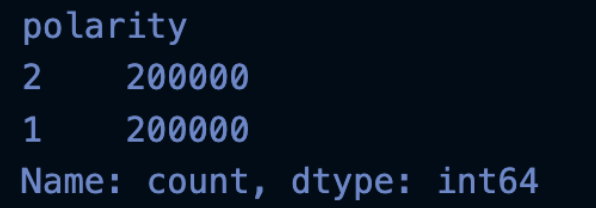
\includegraphics[scale=0.6]{Figures/fig1.png}
        \caption{The distribution of polarity values in the main dataset.}
        \label{fig:enter-label}
    \end{figure}
\end{columns}
}
\end{frame}

%~~~~~~~~~~~~~~~~~~~~~~~~~~~~~~~~~~~~~~~~~~~~~~~~~~~~~~~~~~~~~~~~~~~~~~~~~
\begin{frame}{Second Dataset}
\framesubtitle{HLT Project Proposal}
{\small
\begin{columns}
    \column{0.6\textwidth}
        \begin{table}[]
        \centering
        \begin{tabular}{|l|l|}
            \hline
            \textbf{Column} & \textbf{Description} \\
            \hline
            \texttt{review/score} &$\begin{array}{l}
                 i=\begin{cases}
                1,2 & \text{if the review is negative} \\ 
                3 & \text{if the review is neutral} \\
                4,5 & \text{if the review is positive}
            \end{cases} 
            \end{array}$\\
            \hline 
            \texttt{review/summary} & Title of the review. \\
            \hline
            \texttt{review/text}  & Entire text of the review. \\
             \hline
        \end{tabular}
        %\caption{Amazon Reviews Dataset Structure}
        \label{tab:my_label}
    \end{table}

    \vspace{-0.3cm}
    
    \begin{figure}
        \centering
        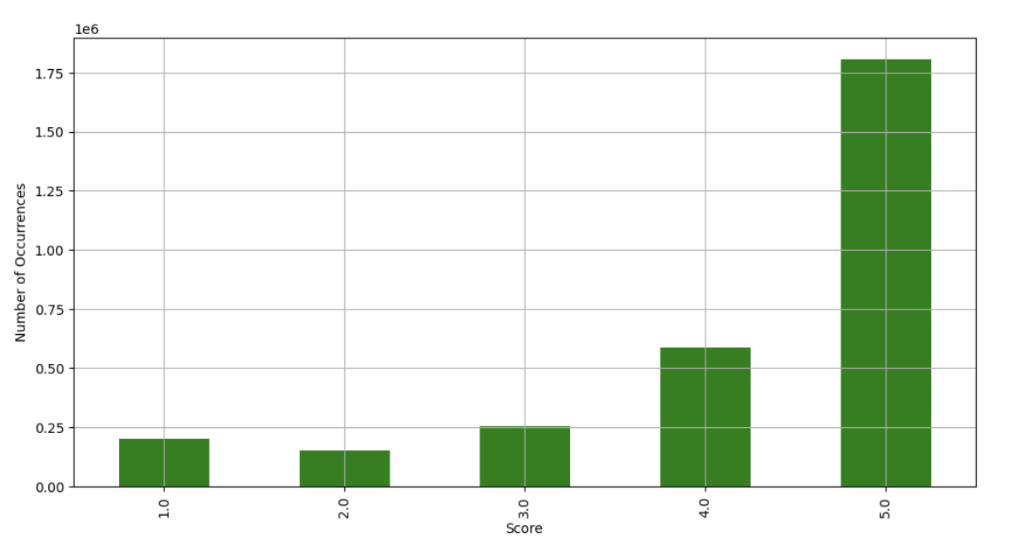
\includegraphics[scale=0.18]{Figures/fig2.png}
        \caption{The distribution of review/score values in the second dataset.}
        \label{fig:enter-label}
    \end{figure}


    \column{0.4\textwidth}
    \begin{itemize}
        \item \textbf{Available at}: \textcolor{teal}{\href{https://www.kaggle.com/datasets/mohamedbakhet/amazon-books-reviews}{Amazon Books Reviews Dataset}}.
        \item \textbf{Context}: The dataset consists of books reviews from Amazon. The dataset contains feedback from approximately 3 million users. For more information: \cite{3}, \cite{4}.
        \item \textbf{Content}: The dataset contains a lot of columns. We will focus only on three columns: review/score, review/summary, review/text
    \end{itemize}

\end{columns}
}
\end{frame}

%~~~~~~~~~~~~~~~~~~~~~~~~~~~~~~~~~~~~~~~~~~~~~~~~~~~~~~~~~~~~~~~~~~~~~~~~~
\begin{frame}{Implementation and Evaluation}
\framesubtitle{HLT Project Proposal}
{\small
\begin{itemize}
\item \textbf{Transformers}: Utilize transformers for binary classification task of sentiment analysis.

\item \textbf{Lexicons}: Incorporate lexicons as additional features to enrich text representation or as labels for pretraining tasks.

\item \textbf{Evaluation Metrics}: Assess model performance using accuracy, precision, recall, F1 score, ROC curves and other metrics, comparing also results across different input types.

\item \textbf{Continuous Improvement}: Plans will evolve as we gain knowledge, ensuring effectiveness and efficiency throughout the project.
\end{itemize}
}
\end{frame}

%~~~~~~~~~~~~~~~~~~~~~~~~~~~~~~~~~~~~~~~~~~~~~~~~~~~~~~~~~~~~~~~~~~~~~~~~~
\begin{frame}{Bibliography}
\framesubtitle{HLT Project Proposal}

\begin{thebibliography}{9}
\setbeamertemplate{bibliography item}[text]

\bibitem{1} J. McAuley and J. Leskovec. \emph{Hidden factors and hidden topics: understanding rating dimensions with review text} RecSys, 2013.

\bibitem{3} R. He, J. McAuley. \emph{Ups and downs: Modeling the visual evolution of fashion trends with one-class collaborative filtering}. WWW, 2016.

\bibitem{4}J. McAuley, C. Targett, J. Shi, A. van den Hengel. \emph{Image-based recommendations on styles and substitutes}. SIGIR, 2015.


\end{thebibliography}
    
\end{frame}

%~~~~~~~~~~~~~~~~~~~~~~~~~~~~~~~~~~~~~~~~~~~~~~~~~~~~~~~~~~~~~~~~~~~~~~~~~
\backmatter
\end{document}

